\clearpage
\section{Robot-Motion Simulation and Delay Experiments}
\label{sec:motion-control}
This retained simulation model is a future software/test environment, not an implemented robot simulator. The mechanical plant maps a steering command $u$ to wheel motion, robot pose, and the next three sensor readings. Its minimum simulation state is the axle-center position $(X,Y)$, heading $\theta$, and actual wheel rim speeds $v_L,v_R$. The caster supports the chassis and follows its motion; it is not a steering actuator. Wheel separation $L_w$, effective rolling radii $R_L,R_R$, sensor forward offset $\ell_s$, sensor spacing, line width, and nominal speed $v_0$ must be recorded as measured quantities or explicit simulation assumptions.

\subsection{Geometry baseline from the September 15 CAD assembly}
The historical simulation geometry is taken from \path{cad_parts/assembly_sep15/main_overview.FCStd}, with the robot assembled, rather than from the exploded copies. Table~\ref{tab:cad-control-dimensions} supplies the simulation baseline. These are dimensions of the saved CAD, not measurements of tire deflection, optical response, or the completed robot. The wheel width/hub and sensor package envelopes remain illustrative.

In the CAD frame, $+Y$ points toward the sensor bar, $+X$ toward the robot's right, and $+Z$ upward. The axle midpoint is $(0,2,-5)$\,mm. Thus the planar body coordinates used in the equations are $x_b=Y_{\mathrm{CAD}}-2$ and $y_b=-X_{\mathrm{CAD}}$, in millimetres. The nominal floor is $Z_{\mathrm{CAD}}=-20$\,mm, tangent to both wheel references and the caster ball.

\begin{table}[H]
\centering
\caption{CAD-derived driving-model dimensions. Convert millimetres to metres in the simulation.}
\label{tab:cad-control-dimensions}
\small
\begin{tabular}{L{4.6cm} L{3.2cm} L{8.4cm}}
\toprule
Quantity & Nominal value & Basis and interpretation \\
\midrule
Wheel-center spacing $L_w$ & 112\,mm & Wheel midplanes at CAD $X=\pm56$\,mm; this is the nominal contact spacing, not the 100\,mm deck width. \\
Wheel radii $R_L,R_R$ & 15\,mm each & 30\,mm diameter references; calibrate effective rolling radii under load. \\
Wheel envelope width & 8\,mm each & Illustrative width; total outside wheel span is 120\,mm. \\
Sensor forward offset $\ell_s$ & 74\,mm & Reference face centers at CAD $Y=76$\,mm, axle at $Y=2$\,mm. \\
Sensor lateral coordinates & $+15.3,\ 0,\ -15.3$\,mm & Left/center/right in the body frame; CAD channels A/B/C. Adjacent pitch 15.3\,mm, outer-center span 30.6\,mm. \\
Axle-to-caster distance & 60\,mm aft & Caster at body $(x_b,y_b)=(-60,0)$\,mm; axle at $(0,0)$. \\
Lower-deck underside clearance & 20\,mm & Main plate underside at CAD $Z=0$; hanging mounts and panels have smaller clearance. \\
Reference sensor-face clearance & 18\,mm & Downward faces at CAD $Z=-2$\,mm; sensor-holder bottom is 9\,mm above the nominal floor. Optical mounting height remains unverified. \\
\bottomrule
\end{tabular}
\end{table}

Use $L_w=0.112$\,m, $R_L=R_R=0.015$\,m, $\ell_s=0.074$\,m and $y_j\in\{0.0153,0,-0.0153\}$\,m initially. Verify that wiring channels A/B/C occupy the correspondingly engraved CAD positions before applying this sign mapping to hardware. Line width, optical footprint, speed, motor gains/lag, and loaded tire behavior still require measurements or declared trial assumptions. In particular, the 18\,mm reference face height is not a validated sensing distance; check the assembled optical height and response before selecting the reflectance model.

Figure~\ref{fig:control-mechanics} defines the mechanical geometry and sign conventions used below. Historical September 15 CAD views appear in Appendix~\ref{app:historical-cad}; the current mechanical package is described in Section~\ref{sec:mechanical-design}.

\begin{figure}[H]
\centering
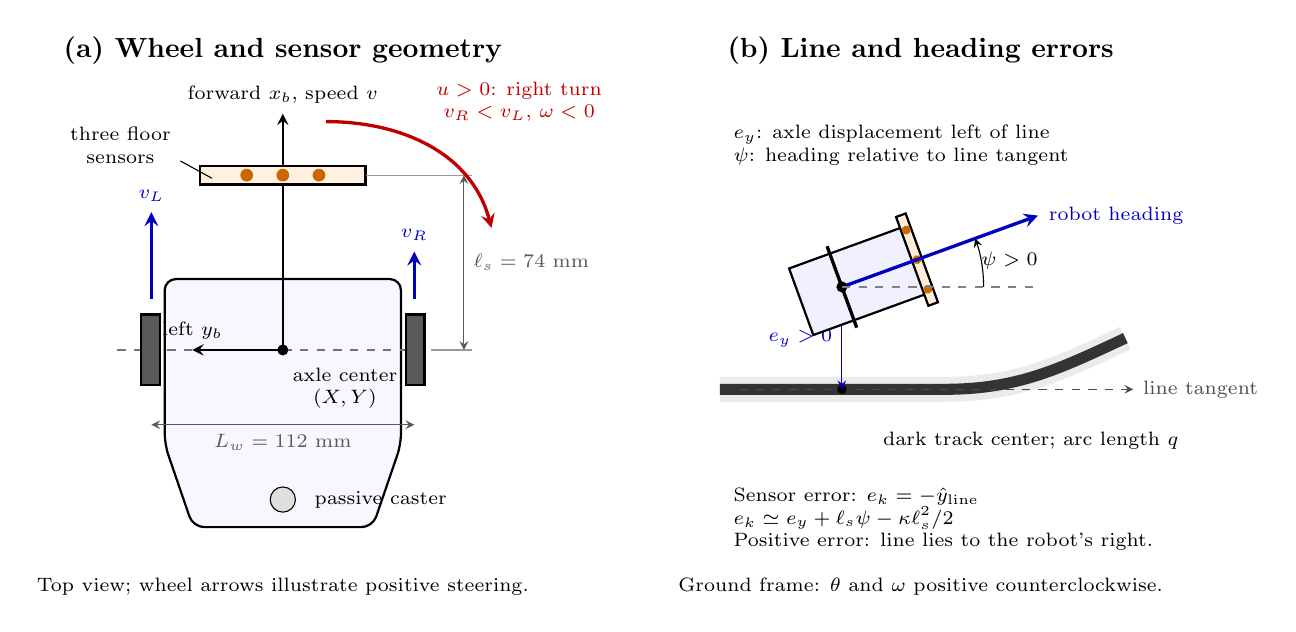
\begin{tikzpicture}[font=\small,>=stealth,
    note/.style={font=\scriptsize,align=center},
    dim/.style={<->,thin,black!65}]
% Panel (a): body coordinates, top view; forward is up.
\node[font=\bfseries] at (0,3.8) {(a) Wheel and sensor geometry};
\draw[thick,fill=blue!3,rounded corners=4pt] (-1.5,0.9) -- (1.5,0.9) -- (1.5,-1.2) -- (1.14,-2.25) -- (-1.14,-2.25) -- (-1.5,-1.2) -- cycle;
\draw[dashed,black!55] (-2.1,0) -- (2.1,0);
\draw[thick,fill=black!65] (-1.8,-0.45) rectangle (-1.56,0.45);
\draw[thick,fill=black!65] (1.56,-0.45) rectangle (1.8,0.45);
\draw[->,very thick,blue!75!black] (-1.67,0.65) -- (-1.67,1.75)
 node[above,note] {$v_L$};
\draw[->,very thick,blue!75!black] (1.67,0.65) -- (1.67,1.25)
 node[above,note] {$v_R$};
\draw[->,thick] (0,0) -- (0,3.0) node[above,note] {forward $x_b$, speed $v$};
\draw[->,thick] (0,0) -- (-1.15,0) node[above,note] {left $y_b$};
\fill (0,0) circle (2pt);
\node[below right,note] at (0,-0.1) {axle center\\$(X,Y)$};
\draw[thick,fill=orange!12] (-1.05,2.1) rectangle (1.05,2.34);
\foreach \xx in {-0.459,0,0.459} {
 \fill[orange!80!black] (\xx,2.22) circle (2.3pt);
}
\node[note,anchor=east] at (-1.3,2.6) {three floor\\sensors};
\draw[thin] (-1.3,2.4) -- (-0.9,2.18);
\draw[dim] (2.3,0) -- (2.3,2.22) node[midway,right,note] {$\ell_s=74$ mm};
\draw[thin,black!40] (1.88,0) -- (2.4,0);
\draw[thin,black!40] (1.05,2.22) -- (2.4,2.22);
\draw[dim] (-1.67,-0.95) -- (1.67,-0.95) node[midway,below,note] {$L_w=112$ mm};
\draw[fill=gray!25] (0,-1.9) circle (0.16cm);
\node[note,anchor=west] at (0.28,-1.9) {passive caster};
\draw[->,very thick,red!75!black] (0.55,2.9) to[out=0,in=105] (2.65,1.55);
\node[note,text=red!75!black] at (3.0,3.15) {$u>0$: right turn\\$v_R<v_L$, $\omega<0$};
\node[note] at (0,-3.0) {Top view; wheel arrows illustrate positive steering.};
% Panel (b): line-relative geometry in a ground frame.
\begin{scope}[shift={(8.1,0)}]
\node[font=\bfseries] at (0,3.8) {(b) Line and heading errors};
% Dark track on a light floor.
\draw[line width=9pt,black!8] (-2.55,-0.5) -- (0.3,-0.5)
 to[out=0,in=205] (2.6,0.15);
\draw[line width=4pt,black!80] (-2.55,-0.5) -- (0.3,-0.5)
 to[out=0,in=205] (2.6,0.15);
\draw[->,dashed,black!70] (-2.3,-0.5) -- (2.7,-0.5)
 node[right,note] {line tangent};
\node[note] at (1.4,-1.15) {dark track center; arc length $q$};
\coordinate (Q) at (-1,-0.5);
\coordinate (P) at (-1,0.8);
\fill (Q) circle (1.7pt);
\draw[dim,blue!75!black] (Q) -- (P) node[midway,left,note] {$e_y>0$};
% Simplified vehicle at positive heading error.
\begin{scope}[shift={(P)},rotate=20]
 \draw[thick,fill=blue!6] (-0.55,-0.45) rectangle (1.05,0.45);
 \draw[very thick] (0,-0.55) -- (0,0.55);
 \draw[thick,fill=orange!15] (0.95,-0.6) rectangle (1.08,0.6);
 \foreach \yy in {-0.4,0,0.4}
   \fill[orange!80!black] (1.015,\yy) circle (1.6pt);
 \draw[->,very thick,blue!75!black] (0,0) -- (2.65,0)
 node[right,note] {robot heading};
\end{scope}
\fill (P) circle (2pt);
\draw[dashed,black!50] (P) -- +(2.5,0);
\draw[->] (0.8,0.8) arc[start angle=0,end angle=20,radius=1.8];
\node[note] at (1.13,1.14) {$\psi>0$};
\node[note,align=left,anchor=west] at (-2.5,2.6)
 {$e_y$: axle displacement left of line\\$\psi$: heading relative to line tangent};
\node[note,align=left,anchor=west] at (-2.5,-2.15)
 {Sensor error: $e_k=-\hat y_{\mathrm{line}}$\\
 $e_k\simeq e_y+\ell_s\psi-\kappa\ell_s^2/2$\\
 Positive error: line lies to the robot's right.};
\node[note] at (0,-3.0) {Ground frame: $\theta$ and $\omega$ positive counterclockwise.};
\end{scope}
\end{tikzpicture}
\caption{Simulation geometry using the historical September 15 baseline (schematic, not to scale). The wheel-speed difference turns the robot; the forward sensor bar observes a combination of lateral displacement, heading error, and line curvature. Panel (b) defines the geometric errors; actual detection is limited by the three-sensor span.}
\label{fig:control-mechanics}
\end{figure}

\subsection{Differential-drive kinematics and turning authority}
Use a ground frame with counterclockwise-positive heading $\theta$ and a body frame with forward and left-positive axes. If $\Omega_L,\Omega_R$ are wheel angular speeds, ideal rolling without slip gives
\begin{align}
 v_L&=R_L\Omega_L,\qquad v_R=R_R\Omega_R,\\
 v&=\frac{v_L+v_R}{2},\qquad
 \omega=\dot\theta=\frac{v_R-v_L}{L_w},\\
 \dot X&=v\cos\theta,\qquad \dot Y=v\sin\theta.
 \label{eq:robot-kinematics}
\end{align}
Thus positive $u$ still means a right turn, but has negative $\omega$ under this heading convention. With ideal wheel tracking of Equation~\eqref{eq:forward-wheel-law},
\begin{equation}
 v=v_0(1-|u|/2),\qquad \omega=-\frac{v_0u}{L_w},\qquad
 \kappa_{\mathrm{robot}}=\frac{\omega}{v}
   =-\frac{u}{L_w(1-|u|/2)}.
 \label{eq:robot-curvature}
\end{equation}
Steering changes both yaw rate and forward speed. For a required clockwise curvature $\kappa_R=-\kappa_{\mathrm{robot}}$, the ideal steady command is
\begin{equation}
 u_{\mathrm{req}}=\frac{L_w\kappa_R}{1+L_w|\kappa_R|/2},\qquad
 |\kappa_R|\le\frac{u_{\max}}{L_w(1-u_{\max}/2)}.
 \label{eq:curvature-authority}
\end{equation}
At $u_{\max}=1$, the current CAD baseline gives a minimum axle-center radius of $L_w/2=56$\,mm and $|\kappa_{\mathrm{robot}}|\le17.86$\,m$^{-1}$. A curve tighter than this is geometrically infeasible under the chosen wheel law regardless of neural latency. Reducing $v_0$ lowers the required response bandwidth, but does not change this ideal curvature limit. These formulas describe axle-center motion; the forward sensor bar traces a different path during a turn. For example, at the 56\,mm minimum axle radius the middle sensor traces a circle of radius $\sqrt{56^2+74^2}\simeq92.8$\,mm about the same instantaneous turn center. A feasible axle trajectory therefore does not by itself ensure that the line remains under the sensors.

As an explicit numerical example, choose $v_0=0.10$\,m/s (a simulation setting, not a measured maximum). Straight motion requires $\Omega_L=\Omega_R=6.67$\,rad/s, about 63.7\,rpm. At $u=1$, the ideal inner wheel stops, $v=0.05$\,m/s and $\omega=-0.893$\,rad/s.

\subsection{Line-relative state and sensor geometry}
Let $q$ be arc length along the dark-track center, $\kappa(q)$ its counterclockwise-positive curvature, $e_y$ the axle-center displacement to the left of the line, and $\psi$ the robot heading minus the line tangent heading. In a region with a unique nearest line point and $1-\kappa e_y>0$,
\begin{equation}
 \dot q=\frac{v\cos\psi}{1-\kappa(q)e_y},\qquad
 \dot e_y=v\sin\psi,\qquad
 \dot\psi=\omega-\kappa(q)\dot q.
 \label{eq:line-relative-motion}
\end{equation}
On a straight line near alignment, $\dot e_y\simeq v\psi$ and $\dot\psi\simeq-v_0u/L_w$. A lateral error alone therefore does not describe the control state: heading error determines how rapidly the line moves across the sensors.

Place sensor $j\in\{1,2,3\}$ at body coordinates $(\ell_s,y_j)$, with $y_j$ positive left and normally symmetric about zero. Its world location is
\begin{equation}
 p_j=\begin{pmatrix}X\\Y\end{pmatrix}
 +\begin{pmatrix}\cos\theta&-\sin\theta\\\sin\theta&\cos\theta\end{pmatrix}
  \begin{pmatrix}\ell_s\\y_j\end{pmatrix}.
 \label{eq:sensor-location}
\end{equation}
The simulator computes each reading from that location, line width, and sensor footprint; it must not supply true $e_y$ or $\psi$ to the Pi. For example, the dark-track response for a dark strip of width $w_{\mathrm{line}}$ with an effective lateral footprint width $w_{\mathrm{spot}}$ can use
\begin{equation}
 z_j=\operatorname{clip}\!\left(
  \frac{w_{\mathrm{line}}/2+w_{\mathrm{spot}}/2-|d_j|}{w_{\mathrm{spot}}};0,1\right),
 \label{eq:reflectance-model}
\end{equation}
where $d_j$ is signed distance from $p_j$ to the nearest line center and $w_{\mathrm{spot}}>0$. This is a simple softened-edge model; replace it with a measured reflectance profile when available, and add illumination offset, noise, clipping, and sample timing separately.

After calibration over the actual light floor and dark track, let $r_j\in[0,1]$ denote calibrated reflectance (light floor: 1; dark track: 0), and define the dark-track weight $z_j=1-r_j$. The simulated $z_j$ above follows this same convention; convert it to $r_j=1-z_j$ for the sensor interface. Appendix~\ref{app:tcrt5000-prototype} describes the current electrical wiring and raw readout; floor/track calibration remains to be measured. Map the physical module positions A, B and C to the chosen $y_j$ coordinates before computing the centroid. A basic line centroid and the sensor error used in Equation~\eqref{eq:sensor-encoder} are
\begin{equation}
 \hat y_{\mathrm{line}}=\frac{\sum_j y_jz_j}{\sum_j z_j},\qquad
 e_k=-\hat y_{\mathrm{line}},\qquad \sum_j z_j>z_{\min}.
 \label{eq:sensor-centroid}
\end{equation}
Positive $e_k$ means the line is to the right of the sensor-bar center and initially calls for positive $u$. Reject the estimate below the saved detection threshold $z_{\min}$; also flag broad or multiple peaks at crossings. Do not convert an undetected line into a zero error. For small heading error and slowly varying curvature,
\begin{equation}
 e_k\simeq e_y+\ell_s\psi-\frac12\kappa\ell_s^2.
 \label{eq:sensor-preview}
\end{equation}
At the CAD offset of 74\,mm, a small heading error of $5^\circ$ contributes approximately 6.46\,mm to the sensor error. The leading curvature term for a 250\,mm-radius line contributes about 10.95\,mm in magnitude. Both are substantial relative to the 15.3\,mm outer-center half-span. The 15.3\,mm sensor pitch also leaves discrete gaps: a line can fall between sensors if the line and sensing footprints are too narrow. Simulate all three readings and their detection threshold; the 30.6\,mm center span is not continuous guaranteed coverage.

The forward bar provides heading sensitivity and geometric preview, while curvature shifts its reading even when the axle is exactly on the line. A single centroid cannot separate $e_y$, $\psi$, and curvature. Timestamped sensor history helps the Pi respond to their evolution. It does not provide absolute position or independently measured wheel speed.

\subsection{Actuator dynamics, traction, and chassis effects}
First simulate ideal wheel speeds. Then replace each speed channel by a bounded empirical actuator model,
\begin{equation}
 \tau_{m,j}\dot v_j+v_j=
 \operatorname{clip}\!\left(
  g_j\max(0,v_j^*(t-T_j)-d_j^{\mathrm{motor}});
  0,v_{j,\max}\right),\qquad j\in\{L,R\}.
 \label{eq:wheel-lag}
\end{equation}
Here $\tau_{m,j}$ is motor/load lag, $T_j$ is command delay, $g_j$ is effective gain, $d_j^{\mathrm{motor}}$ is a speed-equivalent deadband, and $v_{j,\max}$ is the speed limit. This is a model of PWM-to-motion behavior, not a claim that the encoder-free hardware closes a speed loop. Sweep unequal gains and time constants, supply-voltage dependence, and additional slip or external disturbances. At $u=0$, unequal actual wheel speeds still give nonzero yaw.

The ideal kinematic model contains no mass or inertia because it prescribes wheel speeds. Their effects enter the real actuator response and traction. If force-level simulation is needed, a planar extension is
\begin{equation}
 m_{\mathrm{robot}}\dot v=F_L+F_R-F_{\mathrm{res}},\qquad
 I_z\dot\omega=\frac{L_w}{2}(F_R-F_L)-M_{\mathrm{res}},\qquad
 |F_j|\le\mu_{\mathrm{fr}}N_j.
 \label{eq:force-mechanics}
\end{equation}
Here $F_j$ denotes longitudinal tire force and $N_j$ normal load. The coefficient $\mu_{\mathrm{fr}}$ describes friction, and $I_z$ is yaw inertia. The signed terms $F_{\mathrm{res}}$ and $M_{\mathrm{res}}$ represent rolling and caster resistance. Wheel torque and rotational dynamics must also be supplied for that extension; do not impose exact wheel-speed tracking simultaneously. Placing components low and close to the drive axle limits the contributions of their height and distance to load transfer and yaw inertia, while the caster must retain enough load for stable support. Tire compliance, caster friction, an uneven floor, and chassis pitch can change both yaw response and sensor height. Check these effects through measured response or bounded disturbances before attributing tracking failures to the neural model. The CAD-based estimate of about 138\,g is printed plastic only; it is not $m_{\mathrm{robot}}$ and cannot determine $I_z$. Purchased components and their installed masses/locations must be added (Section~\ref{sec:mass-budget}).

For a level floor and a centered lateral CoG, the 60\,mm axle-to-caster lever arm gives the static approximation
\begin{equation}
 \frac{N_C}{m_{\mathrm{robot}}g}=-\frac{x_{\mathrm{CG}}}{0.060},\qquad
 N_L+N_R=m_{\mathrm{robot}}g-N_C,\qquad -0.060<x_{\mathrm{CG}}<0,
 \label{eq:caster-load}
\end{equation}
where $x_{\mathrm{CG}}$ is the forward-positive CoG coordinate in metres and $N_C$ is caster load. Directly over the axle ($x_{\mathrm{CG}}=0$), this ideal static model leaves the caster unloaded. Position the loaded CoG inside the three-contact support triangle and verify the resulting loads; the overview does not contain a measured full-robot CoG.

\subsection{Mechanical interpretation of feedback delay}
During an uncorrected interval $T$, a locally constant heading error and a newly encountered curve give leading-order error magnitudes of order
\begin{equation}
 |\Delta e_y|\sim v|\psi_0|T+\tfrac12|\kappa|v^2T^2,
 \qquad \Delta q\simeq vT.
 \label{eq:delay-distance}
\end{equation}
At the declared straight speed of 0.10\,m/s, the CAD offset corresponds to $\ell_s/v=0.74$\,s of geometric preview; 100\,ms of delay corresponds to 10\,mm of forward travel. These are local estimates, not stability bounds. The geometric preview time is approximately $\ell_s/v$ when $v>0$, but the three sensors do not reveal an arbitrary future curve, so preview is not a guaranteed latency allowance. The line must remain within the finite sensor span while the delayed neural response and wheel dynamics take effect. Sweep speed, curve radius, sensor offset/span, wheel mismatch, and delay jointly. Score axle-center error and sensor-line loss separately, using simulated pose only for evaluation. This distinguishes insufficient turning authority, loss of sensor visibility, actuator limitations, and delayed neural feedback.


